\hypertarget{valores-y-tipos}{%
\section{Values and types}\label{valores-y-tipos}}

\index{valor} \index{tipo} \index{cadena}

A \emph{value} is one of the basic things a program works
with, like a letter or a number. The values we have seen so far are \texttt{1}, \texttt{2} and \texttt{''hello world''}

These values belong to different \emph{types}:

\begin{itemize}[nosep]
    \item \texttt{2} is an \emph{integer}
    \item \texttt{''hello world''} is a \emph{string}, so called because it contains a ``string'' of letters.
\end{itemize}

You (and the interpreter) can identify strings because they are enclosed in quotation marks.

\index{comillas}

The \texttt{print} statement also works for integers. We use
Thonny to start the interpreter and type instructions on the console.

\begin{Verbatim}[frame=single]
>>> print(4)
  4
\end{Verbatim}

If you are not sure what type a value has, the interpreter can tell you.

\begin{Verbatim}[frame=single]
>>> type("hello world")
  <class 'str'>
>>> type(4)
  <class 'int'>
>>> type(3.4)
  <class 'float'>
\end{Verbatim}


Not surprisingly, strings belong to the type \texttt{str} and integers
belong to the type \texttt{int}. Less obviously, numbers with a decimal
point belong to a type called \texttt{float}, because these numbers are
represented in a format called \emph{floating point}.

\index{type} \index{string type} \index{class!str} \index{int type}
\index{class!int} \index{float type} \index{class!float}


What about values like ``17'' and ``3.2''? They look like numbers, but they are in quotation marks like strings.

\index{comillas}
\begin{Verbatim}[frame=single]
>>> type("18")
<class 'str'>
>>> type("4.5")
<class 'str'>
\end{Verbatim}

They're strings.

When you type a large integer, you might be tempted to use commas between groups of three digits, as in 1,000,000. This is not a legal integer in Python, but it is legal:

\index{comillas}
\begin{Verbatim}[frame=single]
>>> print(1,000,000)
  1 0 0
\end{Verbatim}

Well, that's not what we expected at all! Python interprets 1,000,000 as a comma-separated sequence of integers, which it prints with spaces between.

\index{semántico, error} \index{error!semántico}
\index{mensaje de error}

This is the first example we have seen of a semantic error: the code runs without producing an error message, but it doesn't do the "right" thing. (i.e. represent the whole number for one million).

\hypertarget{variables}{%
\section{Variables}\label{variables}}

\index{variable} \index{asignación!sentencia}
\index{sentencia!asignación}

One of the most powerful features of a programming language is the ability to manipulate \emph{variables}. 

\begin{definition}
A \textbf{variable} is a name that refers to a value.
\end{definition}

To create new variables and give them
values we use an \emph{assignment statement}. Below are 3 assignments.

\begin{Verbatim}[frame=single]
>>> message = 'And now for something completely different'
>>> n = 18
>>> pi = 3.1415926535897931
\end{Verbatim}

The first assigns a string to a new variable named \texttt{message}; the second assigns the integer
\texttt{17} to \texttt{n}; the third assigns the (approximate) value of \(\pi\) to \texttt{pi}.

To display the value of a variable, you can use a print statement:

\begin{Verbatim}[frame=single]
>>> print(n)
  18
>>> print(pi)
  3.141592653589793
\end{Verbatim}


The type of a variable is the type of the value it refers to.

\begin{Verbatim}[frame=single]
>>> type(mensaje)
  <class 'str'>
>>> type(n)
  <class 'int'>
>>> type(pi)
  <class 'float'>
\end{Verbatim}


\hypertarget{nombres-de-variables-y-palabras-claves}{%
\section{Variable names and keywords}\label{nombres-de-variables-y-palabras-claves}}

\index{palabra clave}

Programmers generally choose names for their variables that are meaningful and document what the variable is used for.

Variable names can be arbitrarily long. They can contain both letters and numbers, but they cannot start with a number. It is legal to use uppercase letters, but it is a good idea to begin variable names with a lowercase letter (you'll see why later).

The underscore character (\texttt{\_}) can appear in a name. It is often used in names with multiple words, such as
\texttt{my\_name} or \texttt{airspeed\_of\_unladen\_swallow}. Variable names can start with an underscore character, but we generally avoid doing this unless we are writing library code for others to use.

\index{guión-bajo, carácter}

If you give a variable an illegal name, you get a syntax error:

\begin{Verbatim}[frame=single]
>>> 76trombones = 'big parade'
  SyntaxError: invalid syntax
>>> more@ = 1000000
  SyntaxError: invalid syntax
>>> class = 'Advanced Theoretical Zymurgy'
  SyntaxError: invalid syntax
\end{Verbatim}

\texttt{76trombones} is illegal because it begins with a number.
\texttt{more@} is illegal because it contains an illegal character,
\texttt{@}. But what's wrong with \texttt{class}?

It turns out that \texttt{class} is one of Python's \emph{keywords}. The interpreter uses keywords to recognize the structure of the program, and they cannot be used as variable names.

\index{palabra clave}

Python reserves 35 keywords:

\begin{verbatim}
and       del       from      None      True
as        elif      global    nonlocal  try
assert    else      if        not       while
break     except    import    or        with
class     False     in        pass      yield
continue  finally   is        raise-    async
def       for       lambda    return    await
\end{verbatim}

You might want to keep this list handy. If the interpreter complains about one of your variable names and you don't know why, see if it is on this list.

\hypertarget{instrucciones}{%
\section{Statements}\label{sentencias}}

\begin{definition}
A \textbf{statement} is a unit of code that the Python interpreter can execute.
\end{definition}

We have seen two kinds of statements: print being an expression statement and assignment.

\index{sentencia} \index{interactivo, modo} \index{script, modo}

When you type a statement in interactive mode, the interpreter executes it and displays the result, if there is one.

A script usually contains a sequence of statements. If there is more than one statement, the results appear one at a time as the statements execute.

For example, the script

\begin{Verbatim}[frame=single]
print(1)
x = 2
print(x)
\end{Verbatim}

produces the output

\begin{verbatim}
1
2
\end{verbatim}

The assignment statement produces no output.

\hypertarget{operadores-y-operandos}{%
\section{Operators and operands}\label{operadores-y-operandos}}

\index{operador!aritmético} \index{aritmético, operador}
\index{operando} \index{expresión}

\begin{definition}
\textbf{Operators}are special symbols that represent computations like addition and multiplication. The values the operator is applied to are called \textbf{operands}.
\end{definition}

The operators \texttt{+}, \texttt{-}, \texttt{*} , \texttt{/}, and \texttt{**}
perform addition, subtraction, multiplication, division, and exponentiation, as in the following examples:

\begin{Verbatim}[frame=single]
>>> hour = 4+2
>>> minute = 60-1
>>> hour*60+minute
  419
>>> minute/60
  0.9833333333333333
>>> 5**2
  25
>>> (5+9)*(15-8)
  98
\end{Verbatim}

There has been a change in the division operator between Python 2.x and Python 3.x. In Python 3.x, the result of this division is a floating point result:

\begin{Verbatim}[frame=single]
>>> minute = 59
>>> minute/60
  0.9833333333333333
\end{Verbatim}

The division operator in Python 2.0 would divide two integers and truncate the result to an integer:

\begin{Verbatim}[frame=single]
>>> minute = 59
>>> minute/60
  0
\end{Verbatim}


To obtain the same answer in Python 3.0 use floored (\texttt{//} integer) division.

\begin{Verbatim}[frame=single]
>>> minute = 59
>>> minute//60
  0
\end{Verbatim}

In Python 3.0 integer division functions much more as you would expect if you entered the expression on a calculator.

\index{Python 3} \index{Python 2} \index{entera, división}
\index{punto-flotante, división} \index{división!entera}
\index{división!punto-flotante}

\hypertarget{expresiones}{%
\section{Expressions}\label{expresiones}}

\begin{definition}
An \textbf{expression} is a combination of values, variables, and operators. 
\end{definition}

A value all by itself is considered an expression, and so is a variable, so the following are all legal expressions (assuming that the variable \texttt{x} has been assigned a value):

\index{expresión} \index{evaluar}

\begin{Verbatim}[frame=single]
17
x
x + 17
\end{Verbatim}

If you type an expression in interactive mode, the interpreter
\emph{evaluates} it and displays the result:

\begin{Verbatim}[frame=single]
>>> 1 + 1
2
\end{Verbatim}

But in a script, an expression all by itself doesn't do anything! This is a common source of confusion for beginners.

\hypertarget{orden-de-las-operaciones}{%
\section{Order of operations}\label{orden-de-las-operaciones}}

\index{orden de operaciones} \index{reglas de precedencia}
\index{PEMDAS}

\begin{figure}[h]
    \centering
    \includegraphics[width=12cm] {images/pemdas-eng.jpg}
    \caption{Operator Order: PEMDAS}
    \label{fig:PEMDAS}
\end{figure}


When more than one operator appears in an expression, the order of evaluation depends on the \emph{precedence rules}. For mathematical operators, Python follows mathematical convention. The acronym \emph{PEMDAS}  is a useful way to remember the rules (see Figure \ref{fig:PEMDAS}):

\index{paréntesis!invalidar precedencia}

\begin{itemize}
\item
  \emph{P}arentheses have the highest precedence and can be used to force an expression to evaluate in the order you want. Since expressions in parentheses are evaluated first, \texttt{2\ *\ (3-1)} is 4, and \texttt{(1+1)**(5-2)} is 8. You can also use parentheses to make an expression easier to read, as in \texttt{(minutes\ * 100)\ /\ 60}, even if it doesn't change the result.
\item
  La \emph{E}xponentiation has the next highest precedence, so \texttt{2**1+1} is 3, not 4, and \texttt{3*1**3} is 3, not 27.
\item
  \emph{M}ultiplication and \emph{D}ivision have the same precedence, which is higher than \emph{A}ddition and \emph{S}ubtraction, which also have the same precedence. So \texttt{2*3-1} is 5, not 4, and \texttt{6+4/2} is 8, not 5.
\item
  Operators with the same precedence are evaluated from left to right. So the expression \texttt{5-3-1} is 1, not 3, because the \texttt{5-3} happens first and then \texttt{1} is subtracted from \texttt{2}.
\end{itemize}

When in doubt, always put parentheses in your expressions to make sure the computations are performed in the order you intend.

\hypertarget{operador-muxf3dulo}). The syntax is the same as for other operators:

\begin{Verbatim}[frame=single]
>>> quotient = 7 // 3
>>> print(quotient)
  2
>>> remainder = 7 % 3
>>> print(remainder)
  1
\end{Verbatim}


So 7 divided by 3 is 2 with 1 left over.

The modulus operator turns out to be surprisingly useful. For example, you can check whether one number is divisible by another: if
\texttt{x\ \%\ y} is zero, then \texttt{x} is divisible by \texttt{y}.

\index{divisibilidad}

You can also extract the right-most digit or digits from a number. For example, \texttt{x\ \%\ 10} yields the right-most digit of \texttt{x} (in base 10). Similarly,
\texttt{x\ \%\ 100} yields the last two digits.

\hypertarget{operaciones-con-cadenas}{%
\section{String operations
}\label{operaciones-con-cadenas}}

\index{cadena!operación} \index{operador!cadena}

The \texttt{+} operator works with strings, but it is not addition in the mathematical sense. Instead it performs \emph{concatenation}, which means joining the strings by linking them end to end. For example:

\index{concatenación}

\begin{Verbatim}[frame=single]
>>> first = 10
>>> second = 15
>>> print(first+second)
  25
>>> first = '100'
>>> second = '150'
>>> print(first + second)
  100150
\end{Verbatim}

The output of this program is \texttt{100150}.

The \texttt{*} operator also works with strings by multiplying the content of a string by an integer. For example:

\begin{Verbatim}[frame=single]
>>> first = 'Test '
>>> second = 3
>>> print(first * second)
  Test Test Test
\end{Verbatim}

\hypertarget{comentarios}{%
\section{Comments and documentation}\label{comentarios}}

\index{comentarios}

As programs get bigger and more complicated, they get more difficult to read. Formal languages are dense, and it is often difficult to look at a piece of code and figure out what it is doing, or why.

For this reason, it is a good idea to add notes to your programs to explain in natural language what the program is doing. These notes are called comments, and in Python they start with the \texttt{\#} symbol:

\begin{Verbatim}[frame=single]
# compute the percentage of the hour that has elapsed
percentage = (minutes * 100) / 60
\end{Verbatim}

In this case, the comment appears on a line by itself. You can also put comments at the end of a line:

\begin{Verbatim}[frame=single]
percentage = (minutes * 100) / 60     # percentage of an hour
\end{Verbatim}

Everything from the \texttt{\textbackslash{}\#} to the end of the line is ignored; it has no effect on the program.

Comments are most useful when they document non-obvious features of the code. It is reasonable to assume that the reader can figure out \emph{what} the code does; it is much more useful to explain \emph{why}.

This comment is redundant with the code and useless:

\begin{Verbatim}[frame=single]
v = 5     # assign 5 to v
\end{Verbatim}

This comment contains useful information that is not in the code:

\begin{Verbatim}[frame=single]
v = 5     # velocity in meters/second.
\end{Verbatim}

Good variable names can reduce the need for comments, but long names can make complex expressions hard to read, so there is a trade-off.

\hypertarget{elecciuxf3n-de-nombres-de-variables-mnemuxf3nicos}{%
\section{Choosing mnemonic variable names}\label{elecciuxf3n-de-nombres-de-variables-mnemuxf3nicos}}

\index{mnemónico}

As long as you follow the simple rules of variable naming, and avoid reserved words, you have a lot of choice when you name your variables. In the beginning, this choice can be confusing both when you read a program and when you write your own programs. For example, the following three programs are identical in terms of what they accomplish, but very different when you read them and try to understand them.

\begin{Verbatim}[frame=single]
a = 35.0
b = 12.50
c = a * b
print(c)
\end{Verbatim}

\begin{Verbatim}[frame=single]
hours = 35.0
rate = 12.50
pay = hours * rate
print(pay)
\end{Verbatim}

\begin{Verbatim}[frame=single]
x1q3z9ahd = 35.0
x1q3z9afd = 12.50
x1q3p9afd = x1q3z9ahd * x1q3z9afd
print(x1q3p9afd)
\end{Verbatim}

The Python interpreter sees all three of these programs as \emph{exactly the same} but humans see and understand these programs quite differently. Humans will most quickly understand the \emph{intent } of the second program because the programmer has chosen variable names that reflect their intent regarding what data will be stored in each variable.

We call these wisely chosen variable names ``mnemonic variable names''. The word
\emph{mnemonic} means  ``memory aid''.
We choose mnemonic variable names to help us remember why we created the variable in the first place.

While this all sounds great, and it is a very good idea to use mnemonic variable names, mnemonic variable names can get in the way of a beginning programmer's ability to parse and understand code. This is because beginning programmers have not yet memorized the reserved words (there are only 33 of them) and sometimes variables with names that are too descriptive start to look like part of the language and not just well-chosen variable names.

Take a quick look at the following Python sample code which loops through some data. We will cover loops soon, but for now try to just puzzle through what this means:

\begin{Verbatim}[frame=single]
for word in words:
    print(word)
\end{Verbatim}

What is happening here? Which of the tokens (for, word, in, etc.) are reserved words and which are just variable names? Does Python understand at a fundamental level the notion of words? Beginning programmers have trouble separating what parts of the code \emph{debe} be the same as this example and what parts of the code are simply choices made by the programmer.

The following code is equivalent to the above code:

\begin{Verbatim}[frame=single]
for slice in pizza:
    print(slice)
\end{Verbatim}

It is easier for the beginning programmer to look at this code and know which parts are reserved words defined by Python and which parts are simply variable names chosen by the programmer. It is pretty clear that Python has no fundamental understanding of pizza and slices and the fact that a pizza consists of a set of one or more slices.

But if our program is truly about reading data and looking for words in the data, \texttt{pizza} and \texttt{slice} are very un-mnemonic variable names. Choosing them as variable names distracts from the meaning of the program.

After a pretty short period of time, you will know the most common reserved words and you will start to see the reserved words jumping out at you:

\begin{python}[frame=single]
for word in words:
    print(word)
\end{python}


The parts of the code that are defined by Python
(\pythoninline{for},
\pythoninline{in}, 
\pythoninline{print}, 
and \pythoninline{:}) are in bold, and the programmer-chosen variables (\texttt{word} and
\texttt{words}) are not in bold. Many text editors are aware of Python syntax and will color reserved words differently to give you clues to keep your variables and reserved words separate. After a while you will begin to read Python and quickly determine what is a variable and what is a reserved word.

\hypertarget{depuraciuxf3n}{%
\section{Debugging}\label{depuraciuxf3n}}

\index{depuración}

At this point, the syntax error you are most likely to make is an illegal variable name, like \texttt{class} and
\texttt{yield},  which are keywords, or \texttt{odd\textasciitilde{}job} and \texttt{US\$}, which contain illegal characters.

\index{sintaxis, error} \index{error!sintaxis}

If you put a space in a variable name, Python thinks it is two operands without an operator:

\begin{Verbatim}[frame=single]
>>> bad name = 5
  File "<pyshell>", line 1
    bad name = 5
           ^
SyntaxError: invalid syntax
\end{Verbatim}

\begin{Verbatim}[frame=single]
>>> month = 09
  File "<pyshell>", line 1
    month = 09
             ^
SyntaxError: invalid token
\end{Verbatim}

For syntax errors, the error messages don't help much. The most common messages are
\texttt{SyntaxError:\ invalid\ syntax} and
\texttt{SyntaxError:\ invalid\ token}, neither of which is very informative.

\index{mensaje de error} \index{use before def} \index{exception}
\index{runtime error} \index{error!runtime}

The runtime error you are most likely to make is a "use before def;" that is, trying to use a variable before you have assigned a value. This can happen if you spell a variable name wrong:

\begin{Verbatim}[frame=single]
>>> principal = 327.68
>>> interest = principle * rate
Traceback (most recent call last):
  File "<pyshell>", line 1, in <module>
NameError: name 'principle' is not defined
\end{Verbatim}

Variables names are case sensitive, so \texttt{LaTeX} is not the same as \texttt{latex}.

\index{sensibilidad a mayúsculas, nombres de variables}
\index{semántico, error} \index{error!semántico}

At this point, the most likely cause of a semantic error is the order of operations. For example, to evaluate \(\frac{1}{2 \pi}\),
you might be tempted to write

\begin{Verbatim}[frame=single]
>>> 1.0 / 2.0 * math.pi
  1.5707963267948966
>>> 1.0 / (2.0 * math.pi)
  0.15915494309189535
\end{Verbatim}

But the division happens first, so you would get \(\pi / 2\), which is not the same thing! There is no way for Python to know what you meant to write, so in this case you don't get an error message; you just get the wrong answer.

\index{orden de operaciones}

\section{Asking the user for input}

Most of the programs we implement do 3 things:
\begin{enumerate}[nosep]
\item receive ({\em input data}) (for example via the keyboard)
\item do something with this data, for example perform some type of computing
\item display the result as an ({\em output data}) (for example through the screen)
\end{enumerate}

Sometimes, the keyboard/screen combination is known by the name of {\em console} by which both are identified indistinctly. Like the Thonny console.

1. Data entry is done using the \verb+input+ instruction as in the following example:
\begin{python}[frame=single]
     a = int(input("Enter a number: "))
\end{python}
Through this instruction we ask the user to enter a data by keyboard. Obviously, the data entered by keyboard will have to be
stored it somewhere in memory, that is, in a variable.
The previous instruction indicates that the data entered by the console will be interpreted as an integer (\verb+int+) and will be stored in the variable \verb+a+.

2. Calculating the square of the number in \verb+a+ is an example of a computation:

\begin{python}[frame=single]
     square = a * a
\end{python}

This statement calculates the square of \verb+a+ and stores the result in the variable \verb+square+.

3. Display a result can be done with the \verb+print+ command, such as:

\begin{python}[frame=single]
     print("The square is: ", square)
\end{python}

Run this program in the console to test it, for example:
\begin{Verbatim}[frame=single, label={\em example of execution}]
>>> %Run 
  Enter a number: 5
  The square is: 25
\end{Verbatim}

Note that the program must work for any number entered by the user. When we write programs that we can interact with via the console, we can test our program by entering test input data via the keyboard and checking the resulting output on the screen.
To test our program and see if it works for other numbers as well, we could run the following tests through the console:

\begin{Verbatim}[frame=single, label={\em do more tests}]
>>> %Run 
  Enter a number: 0
  The square is: 0
>>> %Run 
  Enter a number: -6
  The square is: 36
>>> %Run 
  The square is: 1000000
  The square is: 1000000000000
\end{Verbatim}

\section{More about the print function and strings}

Strings are used to display text on the screen at any time through print statements.
%
See the following program \verb|area.py|:\\

\begin{python}
print("Program for calculating the area of a square.")
side = int(input("What is the lenth of the side (in cm): "))
area = side * side
print ('The area of a square with side',side, "is", area, 'cm2.')
print ('Thank you for using the program.')
\end{python}



As you can see, strings can be written with single or double quotes.

The first occurrence of \verb+print+ displays a message informing the user of the purpose of the program.
%
The second occurrence of \verb+print+ displays 4 things on the screen:

\begin{enumerate}[nosep]
    \item the text \verb|The area of a square with side|
    \item the value of the side variable
    \item the text \verb|is|
    \itemthe value of the area variable
\end{enumerate}

The \verb+print+ function can display more than one value on the same line: the values to be displayed are enclosed in parentheses and separated by commas.
%
Finally, the last occurrence of \verb+print+ causes a thank you and farewell text to be displayed.

Result when we execute a test of our program:

\begin{Verbatim}[frame=single]
>>> %Run area.py
  Program for calculating the area of a square.
  What is the lenth of the side (in cm): 5
  The area of a square with side 5 is 25 cm2.
  Thank you for using the program.
\end{Verbatim}

\section{Formatting the output: the {\em format} function}
Learning to display formatted information is essential for the user to find
attractive the way you see the results. The format method of strings provides us with a fundamental tool.

Python has 2 ways to format strings:
(1) with the \% operator, and (2) interpolate values using the \texttt{format} function.
%
Here we only describe in more detail how to interpolate values in a string, that is, to substitute a special mark for the value of an expression. Take a look at this instruction:

\begin{figure}[h]
    \centering
    \includegraphics[width=11cm]{images/int1.png}
    \caption{Interpolating a value in a string}
    \label{fig:print-marcas}
\end{figure}

\begin{figure}[h]
    \centering
    \includegraphics[width=0.85\textwidth]{images/int2.png}
    \caption{Interpolating values in a string}
    \label{fig:print-marcas}
\end{figure}



\begin{Verbatim}[frame=single]
>> "The number {0} has been interpolated".format(1.23)
  The number 1.23 has been interpolated
\end{Verbatim}

The {0} character has been replaced by 1.23 (see Figure \ref{fig:print-marcas}).
%
We can interpolate more than one value with a single call to format:

\begin{Verbatim}[frame=single]
>> "The numbers {0} and {1} have been interpolated".format(1.23,9.9999)
  The number 1.23 and 9.9999 have been interpolated
\end{Verbatim}

Each mark of the form \verb|{n}|, where \verb|n| is an integer, it is replaced by a format argument: the \verb|{0}| has been replaced by the first argument and the \verb|{1}| for the second. In general, the \verb|{n}| is replaced by the (n+1)-th argument. You'll get used to a basic Python principle by now: all sequences start at zero (and not just Python: C, Java, and most other commonly used languages also share that principle).

The marks can be arranged within the string in any order you like:

\begin{Verbatim}[frame=single]
>> "The numbers {1} and {0} have been interpolated".format(1.23,9.9999)
  The number 9.9999 and 1.23 have been interpolated
\end{Verbatim}

The marks can be modified to control the appearance of the information. Let's imagine we want to display float values rounded to one decimal place:

\begin{Verbatim}[frame=single]
>> "The numbers {0:.1f} y {1:.1f} have been interpolated".format(1.23,9.9999)
  The numbers 1.2 y 10.0 have been interpolated
\end{Verbatim}


Markups contain format specifiers, and have this structure:

\begin{verbatim}
    {[position]:[flags][minimumwidth][.precision][type code]}
\end{verbatim}

  
Where
\begin{itemize}
\item position: the position of the argument to format:
0 for the first argument and position 1 for the second, etc.

\item type code: character that indicates the type of representation that is desired. It is different depending on the data type of the value. Here are some of its possible values:
\begin{itemize}
\item[*] integer numbers:
\begin{itemize}
\item character d: in base ten (this is the default value).
\item character b: in binary.
\item character c: as Unicode character.
\item character o: in octal.
\item character x: in hexadecimal.
\item character n: the same as d, but as a number adapted to the local culture (in Spanish, for example, the thousands separator is a period and in English it is with a comma).
\end{itemize}
\item[*] floating numbers:
\begin{itemize}
\item  character g: notation in general format, which is only exponent for large numbers (it is the default value).

\item  character e: exponent notation.

\item  character f: fixed point notation.

\item  character n: the same as g, but as a number adapted to the local culture (in Spanish, for example, decimals come after a comma, and in English after a point).

\item  character \%: displays the number multiplied by 100, in f format, and followed by a percent symbol.
\end{itemize}
\end{itemize}


\item minimumwidth - The minimum size. When the size of the argument is less than the minimum, the missing characters will be completed by padding with spaces.

\item .precision: number of decimals with which we want to represent a floating number.

\item flags: there are for example for alignment:
\begin{itemize}
\item \verb|'<'| - align left within spaces (this is the default).
\item \verb|'>'| - align to the right within the available space.
\item \verb|'^'| - forces the field to center within the spaces.
\end{itemize}
\end{itemize}


We will look at some examples below.
%En Poliformat hay un fichero con muchos ejemplos de formatos de salida.


\begin{Verbatim}[frame=single]
>>> txt = "The binary version of {0} is {0:b}"
>>> print(txt.format(5))
  The binary version of 5 is 101

>>> txt = "The hexadecimal version of {0} is {0:x}"
>>> print(txt.format(32))
  The hexadecimal version of 32 is 20
  
>>> txt = "The price is {:.2f} euros."
>>> print(txt.format(45))
  The price is 45.00 euros.

>>> txt = "The price is {:.4f} euros."
>>> print(txt.format(45))
  The price is 45.0000 euros.

>>> txt = "The price is {:.4e} euros."
>>> print(txt.format(45))
  The price is 4.5000e+01 euros.

>>> txt = "The percentage is {:%}"
>>> print(txt.format(0.25))
  The percentage is 25.000000%

>>> txt = "The percentage is {:.1%}"
>>> print(txt.format(0.25))
  The percentage is 25.0%  
\end{Verbatim}

And below more examples on alignment:

\begin{small}
\begin{Verbatim}[frame=single]
>>> txt = "Left alignment {0:<8} of the argument, width 8.".format(49)
print(txt)

Left alignment 49       of the argument, width 8.

>>> txt = "Right alignment {0:>7} of the argument, width 7.".format(49)
print(txt)

Right alignment      49 of the argument, width 7.

>>> txt = "Center alignment {0:^6} of the argument, width 6.".format(49)
print(txt)

Center alignment   49   of the argument, width 6.

>>> txt = "Left alignment {0:a<9} of the argument, width 9, fill con a.".format(49)
print(txt)

Left alignment 49aaaaaaa of the argument, width 9, fill with a.

>>> txt = "Right alignment {0:*>8} of the argument, width 8, fill with *.".format(49)
print(txt)

Right alignment ******49 of the argument, width 8, fill with *.

>>> txt = "Center alignment {0:-^10} of the argument, width 10, fill with -.".format(49)
print(txt)

Center alignment ----49---- of the argument, width 10, fill with -.
>>> 
\end{Verbatim}
\end{small}



\section{More about strings}

\subsection{Indexing of strings}

Strings are not like integers or floating point numbers. A string is a \textbf{sequence}, which means that it is an ordered collection of values. Now we are going to learn how to access the characters that make up a string and you will learn about some of the methods that strings provide.
\index{secuencia}

\index{secuencia}
\index{caracter@carácter}
\index{operador!de corchetes}
\index{corchetes!operador de}
A string is a sequence of characters.
You can access characters one at a time with the bracket operator:

\begin{Verbatim}[frame=single]
>>> fruit = 'banana'
>>> letter = fruit[1]
\end{Verbatim}
%
The second statement selects the first character of \texttt{fruit} and assigns it to \texttt{letter}.
%
The expression in the brackets is called \textbf{index}.
The index indicates which character in the sequence you want (hence the name).
%
However, what you get might not be what you expect:

\begin{Verbatim}[frame=single]
>>> letter
  'a'
\end{Verbatim}
%
For most people, the first letter of \verb"'banana'" is \texttt{b}, not \texttt{a}. But for computer scientists, the index is an offset from the beginning of the string, and the offset of the first letter is zero.

\begin{Verbatim}[frame=single]
>>> letter = fruit[0]
>>> letter
'b'
\end{Verbatim}
%
So \texttt{b} is the letter at position 0 of \verb"'banana'", \texttt{a} is at position 1 and \texttt{n} is at position 2. This is reflected in Figure

\begin{figure}[h]
    \centering
    \includegraphics{images/string.eps}
    \caption{String indexing}
    \label{fig:fruta}
\end{figure}


\index{indice@índice!a partir de cero} 
\index{cero, índice
  a partir de}

As an index, you can use an expression containing variables and operators:
\index{indice@índice}

\begin{Verbatim}[frame=single]
>>> i = 1
>>> fruit[i]
'a'
>>> fruit[i+1]
'n'
\end{Verbatim}
%

But the index value has to be an integer. Otherwise, you get:
\index{excepción!TypeError}
\index{TypeError}

\begin{Verbatim}[frame=single]
>>> letter = fruit[1.5]
TypeError: string indices must be integers
\end{Verbatim}
%

\subsection{Negative indices}

You can use negative indices, which go from the right to the left of the string, as you can see in Figure \ref{fig:string-negativa} and \ref{fig:string-hola}. The expression \texttt{fruit[-1]} returns the last letter, \texttt{fruit[-2]} returns the penultimate, and so on.
\index{indice@índice!negativo}
\index{negativo, índice}

\begin{figure}[h]
    \centering
    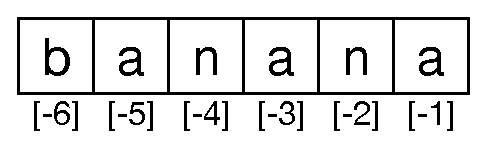
\includegraphics{images/string-negatief}
    \caption{Using negative indices}
    \label{fig:string-negativa}
\end{figure}


\begin{Verbatim}[frame=single]
>>> fruit = 'banana'
>>> fruit[-2]
  'n'
>>> fruit[-5]
  'a'
  
>>> s = 'Hello World'
>>> s[-7]
'o'
>>> s[-2]
'l'
\end{Verbatim}


\subsection{The \texttt{len} function}
\index{función!len}
\index{len, función}

\texttt{len} is a Python built-in function that returns the number of characters in a string:

\begin{Verbatim}[frame=single]
>>> fruit = 'banana'
>>> len(fruit)
6
\end{Verbatim}
%
To get the last letter of a string, you might be tempted to try something like this:
\index{excepción!IndexError}
\index{IndexError}

\begin{Verbatim}[frame=single]
>>> length = len(fruit)
>>> last = fruit[length]
IndexError: string index out of range
\end{Verbatim}
%
The reason for the \texttt{IndexError} is that there is no letter in \texttt{banana} with index 6. Since we started counting from zero, the six letters are numbered from 0 to 5. To get the last character, you have
to subtract 1 from \texttt{length}:

\begin{Verbatim}[frame=single]
>>> last = fruit[length-1]
>>> last
'a'
\end{Verbatim}

\subsection{The slicing operator}

\label{slice}
\index{operador!de trozo} \index{trozo!operador} \index{indice@índice!de trozo}
\index{cadena!trozo de} \index{trozo de cadena} \index{slice}

A segment of a string is called {\em slice}. Selecting a slice is similar to selecting a character:

\begin{Verbatim}[frame=single]
>>> s = 'Hello World'
>>> s[0:5]
  'Hello'
>>> s[6:10]
  'Worl'
\end{Verbatim}
%
The \texttt{[n:m]} operator returns the part of the string from the ``nth'' character to the ``mth'' character, including the first but excluding the last. This behavior is counter-intuitive, you have to practice it a lot and think about how the indices are (see Figure \ref{fig:string-hola}).

\begin{figure}[h]
\centerline
{\includegraphics[scale=0.8]{images/string-hello.jpg}}
\caption{Hello World indices}
\label{fig:string-hola}
\end{figure}

If you omit the first index (before the colon), the chunk starts at the beginning of the string. If you omit the second index, the chunk goes to the end of the string:

\begin{Verbatim}[frame=single]
>>> fruit = 'banana'
>>> fruit[:3]
  'ban'
>>> fruit[3:]
  'ana'
\end{Verbatim}
%
If the first index is equal to or greater than the second, the result is an \textbf{empty string}, represented by two quotes:
\index{comillas}

\begin{Verbatim}[frame=single]
>>> fruit = 'banana'
>>> fruit[3:3]
  ''
>>> fruit[4:2]
  ''
\end{Verbatim}
%
An empty string contains no characters and has length 0, but other than that it's the same as any other string.

Continuing with this example, what do you think \texttt{fruit[:]} means? Try it and see.
\index{trozo!copia de}
\index{copia!de trozo}


\subsection{Strings are immutable}
\index{mutabilidad}
\index{inmutabilidad}
\index{cadena!inmutable}

It's tempting to use the \texttt{[]} operator on the left side of an assignment, with the intention of changing a character in a string. For example:
\index{TypeError}
\index{excepción!TypeError}

\begin{Verbatim}[frame=single]
>>> greeting = 'Hello World'
>>> greeting[0] = 'J'
  TypeError: 'str' object does not support item assignment
\end{Verbatim}
%
The ``object'' in this case is the string, and the ``ítem'' is the character you tried to assign. The reason of the error is that strings are \textbf{immutable}, which means you can't change a string that already exists. The best you can do is create a new string that is a variation of the original:

\begin{Verbatim}[frame=single]
>>> greeting = 'Hello World'
>>> new_greeting = 'J' + greeting[1:]
>>> new_greeting
  'Jello World'
\end{Verbatim}
%
This example concatenates a new first letter with a \texttt{greeting} slice. It has no effect on the original string.
\index{concatenación}


\subsection{String handling methods}

Strings provide methods that perform a variety of useful operations. For example, the \texttt{upper} method takes a string and returns a new string with all uppercase letters.


\begin{Verbatim}[frame=single]
>>> word = 'banana'
>>> new_word = word.upper()
>>> new_word
  'BANANA'
\end{Verbatim}

Here is a table with other methods that may be useful:

\includegraphics[width=\textwidth]{images/methods-string.png}


\hypertarget{glosario}{%
\section*{Glossary}\label{glosario}}

\begin{description}
\item[assignment]
A statement that assigns a value to a variable.
\end{description}

\index{asignación}

\begin{description}
\item[string]
A type that represents sequences of characters.
\end{description}

\index{cadena}

\begin{description}
\item[concatenate]
Join two operands, one after the other.
\end{description}

\index{concatenación}

\begin{description}
\item[comment]
Information in a program that is put out for other programmers (or anyone else reading the source code), and has no effect on the execution of the program.
\end{description}

\index{comentarios}

\begin{description}
\item[integer division]
The operation that divides two numbers and truncates the fractional part.
\end{description}

\index{división!entera}

\begin{description}
\item[integer]
A type that represents integers.
\end{description}

\index{entero}

\begin{description}
\item[evaluate]
Simplify an expression by performing the operations in order to obtain a single value.
\end{description}

\index{evaluar}

\begin{description}
\item[expression]
A combination of variables, operators, and values that represent a single result value.
\end{description}

\index{expresión}

\begin{description}
\item[mnemonic]
An aid to memorize. We often give variables mnemonic names to help us remember what is stored in them.
\end{description}

\index{mnemónico}

\begin{description}
\item[keyword]
A reserved word that is used by the compiler to parse a program; keywords such as \texttt{if}, \texttt{def} and \texttt{while} cannot be used as variable names.
\end{description}

\index{palabra clave}

\begin{description}
\item[floating point]
A type that represents numbers with a decimal part.
\end{description}

\index{punto-flotante}

\begin{description}
\item[operator]
A special symbol that represents a simple calculation, such as addition, multiplication, or string concatenation.
\end{description}

\index{operador}

\begin{description}
\item[modulus operator]
An operator, represented by a percent sign (\texttt{\%}), that works on integers and returns the remainder when one number is divided by another.
\end{description}

\index{módulo, operador} \index{operador!módulo}

\begin{description}
\item[operand]
One of the values with which an operator operates.
\end{description}

\index{operando}

\begin{description}
\item[precedence rules]
The set of rules that sets the order in which expressions involving multiple operators are evaluated.
\end{description}

\index{reglas de precedencia} \index{precedencia}

\begin{description}
\item[statement]
A section of code that represents a command or action. So far, the only statements we've seen are assignments and print statements.
\end{description}

\index{sentencia}

\begin{description}
\item[type]
A category of values. The types we've seen so far are integers (type \texttt{int}), floating-point numbers (type \texttt{float}), and strings (type \texttt{str}).
\end{description}

\index{tipo}

\begin{description}
\item[value]
One of the basic units of data, such as a number or a string, that a program manipulates.
\end{description}

\index{valor}

\begin{description}
\item[variable]
A name that refers to a value.
\end{description}

\index{variable}

\newpage

\hypertarget{ejercicios}{%
\section*{Open response exercises}\label{ejercicios}}
\addcontentsline{toc}{section}{Open response exercises}

\begin{enumerate}
%\setlength{\itemindent}{1.3cm}
\setlength\itemsep{2em}

\item Given the following expression in Python

\pythoninline{7 + 5 * 4 / 3 + 5}

What is your result?

Change it using parentheses so that its result is 6


\respuesta{
18,66\\
((7 + 5) * 4) /(3+5)
}



\item Write a Python statement that assigns to a variable the arithmetic mean of the variables a, b, and c (integer variables).

\respuesta{
\pythoninline{media = (a + b + c) / 3}
}

\item Write the Python instructions that allow to calculate over 2 variables \pythoninline{days} and \pythoninline{hours} the number of days and hours to which a certain number of hours is equivalent (totalHours). For example,

- if totalHours is equal to 60, then days will be equal to 2 and hours equal to 12;

- if totalHours is equal to 25, then days will be equal to 1 and hours equal to 1.

%\begin{pythonrespuesta}
%dias = totalHoras // 24
%horas = totalHoras   24
%\end{pythonrespuesta}


\item Assume we have the following assignment statements:
\begin{python}
    width = 17
    height = 12.0
\end{python}

For each of the expressions below, write the value of the expression and the type (of the expression value).

(a)  \pythoninline{width/2}

(b)   \pythoninline{width/2.0}

(c)   \pythoninline{height/3}

(d)   \pythoninline{height * 5}

(e)   \pythoninline{width * 4}

\respuesta{
a.  \pythoninline{8.5 - float}

b.  \pythoninline{8.5 - float}

c.  \pythoninline{4.0 - float}

d.  \pythoninline{60.0 - float}

e.  \pythoninline{68 - int}
}


\item Write a Python program that uses input to ask the user for his/her name and then greet him/her. Something like:


\begin{Verbatim}[frame=single, label={\em examples and possible execution tests}]
>>> %Run
  Enter your name: Tanja
  Hi Tanja!
\end{Verbatim}

\respuesta{
Mira el fichero  \pythoninline{respuestas11-15.py}
}
%MERK-OP de numering is veranderd!


\item Write a Python program that reads an amount in miles from the keyboard as an integer and displays its equivalent in kilometers on the screen. Note that 1 mile is 1.609344 kilometers.

\begin{Verbatim}[frame=single, label={\em examples and possible execution tests}]
>>> %Run
  How many miles? 200
  in km is 321.8688
\end{Verbatim}

\respuesta{
Mira el fichero  \pythoninline{respuestas11-15.py}
}


\item Given two variables \verb+a+ and \verb+b+, make a Python program that allows the user to enter two values in the variables, exchange their values and display them on the screen. Running the program should result in the following:
\begin{Verbatim}[frame=single, label={\em example of execution}]
>>> %Run 
  Enter the value of the variable a: 4
  Enter the value of variable b: 2
  The value of a is 2
  The value of b is 4
\end{Verbatim}
Assuming that 4 and 2 are the values entered by the user.
This should work for any pair of values entered by the user.

Run tests through the console and check the output. Does your program work with negative numbers? Does it work with letters? Does it work with real numbers? Can the variables \verb+a+ and \verb+b+ have different types? Should your program work for all these cases?




\item Write a Python program that reads the number of dogs in a park from the keyboard. Use 3 variables to calculate the number of heads, legs, and ears in the park. Print the result on the screen.

\begin{Verbatim}[frame=single, label={\em examples and possible execution tests}]
>>> %Run
  How many dogs are there? 15
  There are 15 heads, 60 legs and 30 ears.
>>> %Run
  How many dogs are there? 1
  There is 1 head, 4 legs and 2 ears.
\end{Verbatim}

\respuesta{
Mira el fichero  \pythoninline{respuestas11-15.py}
}

\item Write a Python program that asks the user for the number of hours worked and the hourly rate. Returns the gross salary.

\begin{Verbatim}[frame=single, label={\em examples and possible execution tests}]
>>> %Run
  How many hours? 10
  What is the gross hourly rate? 65
  Gross salary is: 650.0
>>> %Run
  How many hours? 13.5
  What is the gross rate per hour? 10
  Gross salary is: 135.0
\end{Verbatim}
\respuesta{
Mira el fichero  \pythoninline{respuestas11-15.py}
}

\item Implement a program that calculates the temperature in degrees Celsius from the temperature in degrees Fahrenheit. The formula is as follows:
\begin{displaymath}
  C = \frac{5}{9}(F-32)
\end{displaymath} 
The input to the program is the degrees Fahrenheit entered by the user. We will store this value in a variable, for example \verb+F+. Next, our program calculates the expression given by the formula and stores the result in another variable, for example \verb+C+. The last step will be to print the result to the user.

\begin{Verbatim}[frame=single, label={\em example of execution}]
>>> %Run 
  Enter degrees Fahrenheit: 84
  84.0 degrees Fahrenheit is 28.9 degrees Celsius
\end{Verbatim}

Make more tests of your program to verify its answers using this online converter:

\url{https://www.metric-conversions.org/temperature/fahrenheit-to-celsius.htm}

%TODO
%https://www.geeksforgeeks.org/program-distance-two-points-earth/

\end{enumerate}

\section*{Multiple choice exercises}
\addcontentsline{toc}{section}{Multiple choice exercises} 


Imagine that we define the following String in Python:

\begin{Verbatim}
s = "Hello everyone!"
\end{Verbatim}

\noindent What comes out when we type? ({\color{deepred} \textbf{NOTE}: do not use the Python interpreter to do the multiple choice exercises you will not have it in the exam either})\\


\begin{enumerate}
\item
\begin{Verbatim}
s[-8]
\end{Verbatim}

\begin{choices}
    \choice \verb@'e'@
    \choice \verb@'v'@
    \choice \verb@' '@
    \choice \verb@IndexError@
\end{choices}

%\solution{v}

\item 
\begin{Verbatim}
s[2:6]
\end{Verbatim}

\begin{choices}
    \choice \verb@'llo '@
    \choice \verb@'lo e'@
    \choice \verb@'lo '@
    \choice \verb@'llo'@
\end{choices}


%\solution{'lo '}


\item 
\begin{Verbatim}
s[1:4:2]
\end{Verbatim}

\begin{choices}
    \choice \verb@'el'@
    \choice \verb@'Hell'@
    \choice \verb@'el '@
    \choice \verb@'Hl '@
\end{choices}

%\solution{'el'}


\item 
\begin{Verbatim}
s[:5]
\end{Verbatim}

\begin{choices}
    \choice \verb@'ello '@
    \choice \verb@'Hello'@
    \choice \verb@' re'@
    \choice \verb@'Hoen'@
\end{choices}

%\solution{'Hello '}

\item 
\begin{Verbatim}
s[10:5:-1]
\end{Verbatim}


\begin{choices}
    \choice \verb@'yreve'@
    \choice \verb@'oyrev@
    \choice \verb@'o eve'@
    \choice \verb@IndexError@
\end{choices}


%\solution{'yreve'}

\item 
\begin{Verbatim}
s + ' Hi!'
\end{Verbatim}

\begin{choices}
    \choice \verb@'Hello everyone! Hi!'@
    \choice \verb@'str +  Hi!'@
    \choice \verb@TypeError: can only concatenate str (not "int") to str@
    \choice \verb@False@
\end{choices}

%\solution{'Hello everyone! Hi!'}

\item 
\begin{Verbatim}
s[len(s) - 4]
\end{Verbatim}

\begin{choices}
    \choice \verb@'y'@
    \choice \verb@'o'@
    \choice \verb@TypeError@
    \choice \verb@IndexError@
\end{choices}

%\solution{'y'}

\item 
\begin{Verbatim}
s[-1:8:-1]
\end{Verbatim}

\begin{choices}
    \choice \verb@'ello ev'@
    \choice \verb@''@
    \choice \verb@'!enoyr'@
    \choice \verb@IndexError@
\end{choices}

%\solution{'!enoyr'}

\item 
\begin{Verbatim}
s[-1:8:-2]
\end{Verbatim}

\begin{choices}
    \choice \verb@'!ny'@
    \choice \verb@'el v'@
    \choice \verb@''@
    \choice \verb@IndexError@
\end{choices}

%\solution{'!ny'}

\item 
\begin{Verbatim}
s[len(s)-1:8:-2]
\end{Verbatim}

\begin{choices}
    \choice \verb@'!ny'@
    \choice \verb@''@
    \choice \verb@TypeError@
    \choice \verb@IndexError@
\end{choices}

%\solution{'!ny'}

\item What is the value of the following expression?

1 + 2 ** 3 * 4

\begin{choices}
    \choice 36
    \choice 4097
    \choice 33 %CORRECT
    \choice 108
\end{choices}

%\solucion{C}

\item Consider the following Python statement:

\begin{python}
x = a + 5 - b
\end{python}

a y b are, and 


a + 5 - b is: 

\begin{choices}
    \choice operands and an expression %CORRECT
    \choice operators and an instruction
    \choice instructions and a condition
    \choice operands and an equation
\end{choices}

\item What is the result of the expression \texttt{22\ \%3}?

\begin{choices}
    \choice 7
    \choice 1 %CORRECT
    \choice 0
    \choice error
\end{choices}

\item Imagine the following expression in Python:

\begin{python}
6 * '=' + 3 * '(O)' + 6 * '='
\end{python}

What's the result?


\begin{choices}
    \choice \verb|'======(O)(O)(O)======'| %CORRECT
    \choice \verb|15|
    \choice \verb|False|
    \choice \verb|'6=3(0)6='|
\end{choices}

\item Imagine the following statement in Python:

\begin{python}
print('%d has %.2d sons' % ("Luis", 4))
\end{python}

What's the result?

\begin{choices}
    \choice TypeError %CORRECT
    \choice \pythoninline{Louis has 04 sons}
    \choice \pythoninline{Louis has 4 sons}
    \choice \pythoninline{Louis has 4.00 sons}
\end{choices}

\item Imagine the following statement in Python:

\begin{python}
print('{1:b} dogs, {2} birds and {3} cats'.format(3,4,5,6))
\end{python}

What's the result?


\begin{choices}
     \choice   \pythoninline{100 dogs, 5 birds y 6 cats} %CORRECT
    \choice \pythoninline{3 dogs, 4 birds y 5 cats}
    \choice \pythoninline{4 dogs, 5 birds y 6 cats}
    \choice IndexError
\end{choices}

\item What is the result of the expression: \verb|3*1**3|?

\begin{choices}
    \choice 3 %CORRECT
    \choice 9
    \choice 1
    \choice 27
\end{choices}


\item What will be the output of the following Python code?

\begin{python}
'%f %s %d you' %(1, 'hello', 4.0)
\end{python}

\begin{choices}
    \choice \pythoninline{'1.000000 hello 4 you'} %CORRECT
    \choice \pythoninline{'1 hello you 4.0'}
    \choice \pythoninline{'1 hello 4.0 you'}
    \choice \pythoninline{'1.0 hello 4.0 you'}
\end{choices}



\end{enumerate}